\subsection{x86}

\subsubsection{\NonOptimizing MSVC}

\RU{Это дает в итоге}\EN{Result} (MSVC 2010):

\lstinputlisting[caption=MSVC 2010]{patterns/08_switch/1_few/few_msvc.asm}

\RU{Наша функция со switch()-ем, с небольшим количеством вариантов, 
это практически аналог подобной конструкции:}
\EN{Our function with a few cases in switch(), in fact, is analogous to this construction:}

\lstinputlisting[label=switch_few_ifelse]{patterns/08_switch/1_few/few_analogue.c}

\index{\CLanguageElements!switch}
\index{\CLanguageElements!if}
\RU{Когда вариантов немного, и мы видим подобный код, невозможно сказать с уверенностью, был ли
в оригинальном исходном коде switch(), либо просто набор if()-ов.}
\EN{If we work with switch() with a few cases, it is impossible to be sure, was it
real switch() in source code, or just pack of if() statements.}
\index{\SyntacticSugar}
\RU{То есть, switch() это синтаксический сахар для большого количества вложенных проверок 
при помощи if().}
\EN{This means, switch() is like syntactic sugar for large number of nested checks constructed using if().}

\RU{В самом выходном коде, в принципе, ничего особо нового для нас здесь, 
за исключением того, что компилятор зачем-то 
перекладывает входящую переменную ($a$) во временную в локальном стеке \TT{v64}
\footnote{Локальные переменные в стеке с префиксом \TT{tv} --- 
так MSVC называет внутренние переменные для своих нужд}.}
\EN{Nothing especially new to us in generated code,
with the exception the compiler moving 
input variable 
$a$ to temporary local variable \TT{tv64}
\footnote{Local variables in stack prefixed with \TT{tv} --- 
that's how MSVC names internal variables for its needs}.}

\RU{Если скомпилировать это при помощи GCC 4.4.1, то будет почти то же самое, даже с максимальной оптимизацией 
(ключ \Othree).}
\EN{If to compile the same in GCC 4.4.1, we'll get almost the same, even with maximal optimization 
turned on (\Othree option).}

\subsubsection{\Optimizing MSVC}

\RU{Попробуем, включить оптимизацию кодегенератора}
\EN{Now let's turn on optimization in} MSVC (\Ox): \TT{cl 1.c /Fa1.asm /Ox}

\label{JMP_instead_of_RET}
\lstinputlisting[caption=MSVC]{patterns/08_switch/1_few/few_msvc_Ox.asm}

\RU{Вот здесь уже все немного по-другому, причем не без грязных хаков.}
\EN{Here we can see some dirty hacks.}

\index{x86!\Instructions!JZ}
\index{x86!\Instructions!JE}
\index{x86!\Instructions!SUB}
\RU{Первое: \TT{а} помещается в \EAX и от него отнимается 0. Звучит абсурдно, но нужно это для того, чтобы проверить, 
0 ли в \EAX был до этого? Если да, то выставится флаг \ZF (что означает что результат отнимания $0$ от числа 
стал $0$) и первый условный переход \JE (\IT{Jump if Equal} или его синоним \JZ ~--- \IT{Jump if Zero}) 
сработает на метку \TT{\$LN4@f}, где выводится сообщение \TT{'zero'}.
Если первый переход не сработал, от значения отнимается по единице, 
и если на какой-то стадии образуется в результате $0$, то сработает соответствующий переход.}
\EN{First: the value of the $a$ variable is placed into \EAX and $0$ subtracted from it. Sounds absurd, but it may needs to check if 
$0$ was in the \EAX register before? If yes, flag \ZF will be set (this also means that subtracting from $0$ is $0$) 
and first conditional jump \JE (\IT{Jump if Equal} or synonym \JZ~---\IT{Jump if Zero}) will be triggered 
and control flow passed to the \TT{\$LN4@f} label, where \TT{'zero'} message is being printed. 
If first jump was not triggered, $1$ subtracted from the input value and if at some stage $0$ will be resulted, 
corresponding jump will be triggered.}

\RU{И в конце концов, если ни один из условных переходов не сработал, управление передается \printf
со строковым аргументом \TT{'something unknown'}.}
\EN{And if no jump triggered at all, control flow passed to the \printf with argument \TT{'something unknown'} string.}

\label{jump_to_last_printf}
\index{\Stack}
\RU{Второе: мы видим две, мягко говоря, необычные вещи: указатель на сообщение помещается в переменную $a$, 
и затем \printf вызывается не через \CALL, а через \JMP. Объяснение этому простое. 
Вызывающая функция заталкивает в стек некоторое значение и через \CALL вызывает нашу функцию. 
\CALL в свою очередь заталкивает в стек адрес возврата (\ac{RA}) и делает безусловный переход на адрес нашей функции. 
Наша функция в самом начале (да и в любом её месте, потому что в теле функции нет ни одной инструкции, 
которая меняет что-то в стеке или в \ESP) имеет следующую разметку стека:}
\EN{Second: we see unusual thing for us: string pointer is placed into the $a$ variable, and 
then \printf is called not via \CALL, but via \JMP. This could be explained simply. 
\Gls{caller} pushing to stack a value and calling our function via \CALL. 
\CALL itself pushing returning address (\ac{RA}) to stack and do unconditional jump to our function address. 
Our function at any point of execution (since it do not contain any instruction moving stack 
pointer) has the following stack layout:}

\begin{itemize}
\item\ESP\EMDASH\RU{хранится}\EN{pointing to} \ac{RA}
\item\TT{ESP+4}\EMDASH\RU{хранится значение $a$}\EN{pointing to the $a$ variable} 
\end{itemize}

\RU{С другой стороны, чтобы вызвать \printf нам нужна почти такая же разметка стека, 
только в первом аргументе нужен указатель на строку. Что, собственно, этот код и делает.}
\EN{On the other side, when we need to call \printf here, we need exactly the same stack 
layout, except of first \printf argument pointing to string. 
And that is what our code does.}

\RU{Он заменяет свой первый аргумент на адрес строки, и затем передает управление \printf, как если бы вызвали не 
нашу функцию \ttf, а сразу \printf. 
\printf выводит некую строку на \gls{stdout}, затем исполняет инструкцию \RET, 
которая из стека достает \ac{RA} и управление передается в ту функцию, 
которая вызывала \ttf, минуя при этом конец ф-ции \ttf.}
\EN{It replaces function's first argument to address of the string and 
jumping to the \printf, as if not our function \ttf was called firstly, but immediately \printf.
\printf printing a string to \gls{stdout} and then execute \RET instruction, which POPping 
\ac{RA} from stack and control flow is returned not to \ttf but rather to the \ttf's \gls{callee}, 
bypassing end of \ttf function.}

\index{\CStandardLibrary!longjmp()}
\newcommand{\URLSJ}{\url{http://en.wikipedia.org/wiki/Setjmp.h}}
\RU{Все это возможно потому что \printf вызывается в \ttf в самом конце. 
Все это чем-то даже похоже на \TT{longjmp()}\footnote{\URLSJ}.
И все это, разумеется, сделано для экономии времени исполнения.}
\EN{All this is possible since \printf is called right at the end of the \ttf function in any case. 
In some way, it is all similar to the \TT{longjmp()}\footnote{\URLSJ} function.
And of course, it is all done for the sake of speed.}

\RU{Похожая ситуация с компилятором для ARM описана в секции}
\EN{Similar case with ARM compiler described in} ``\PrintfSeveralArgumentsSectionName'', 
\RU{здесь}\EN{section, here}~(\ref{ARM_B_to_printf}).

\myparagraph{\olly}

\RU{Так как этот пример немного запутанный, попробуем оттрассировать его в}\EN{Since this example is tricky, 
let's trace it in} \olly.\\
\\
\olly \RU{может распознавать подобные switch()-конструкции, так что он добавляет полезные комментарии}\EN{can 
detect such switch() constructs, so its add some useful comments}.
\EAX \RU{в начале}\EN{is} $2$\EN{ at start}, \RU{это входное значение ф-ции}\EN{that's function's input value}: \figref{fig:switch_few_olly1}\\
\\
$0$ \RU{отнимается от}\EN{is subtracted from} $2$ \InENRU \EAX. 
\RU{Конечно же}\EN{Of course}, \EAX \RU{все еще содержит}\EN{is still contain} $2$.
\RU{Но флаг}\EN{But} \ZF \RU{теперь}\EN{flag is now} $0$, \RU{что означает что последнее вычисленное значение
не было нулевым}\EN{indicating that resulting value is non-zero}:
\figref{fig:switch_few_olly2}.\\
\\
\DEC \RU{исполнилась и}\EN{is executed and} \EAX \RU{теперь содержит}\EN{now contain} $1$. 
\RU{Но}\EN{But} $1$ \RU{не ноль, так что флаг}\EN{is non-zero, so the} \ZF \RU{все еще}\EN{flag is still} $0$:
\figref{fig:switch_few_olly3}.\\
\\
\RU{Следующая}\EN{Next} \DEC \RU{исполнилась}\EN{is executed}. 
\EAX \RU{наконец}\EN{is finally} $0$ \RU{и флаг}\EN{and} \ZF \RU{выставлен, потому что результат --- ноль}\EN{flag
is set, because the result is zero}: \figref{fig:switch_few_olly4}.
\olly \RU{показывает, что условный переход сейчас сработатет}\EN{shows that this jump will be taken now}.\\
\\
\RU{Указатель на строку}\EN{A pointer to the string} ``two'' \RU{сейчас будет записан в стек}\EN{will now be 
written into the stack}:
\figref{fig:switch_few_olly5}.
\RU{Обратите внимание: текущий аргумент ф-ции это $2$ и $2$ прямо сейчас в стеке по адресу}\EN{Please note: 
current argument of the function is $2$ and $2$ is now in the stack at the address} \TT{0x0020FA44}.\\
\\
\MOV \RU{записывает указатель на строку по адресу}\EN{wrote pointer to the string at the address} 
\TT{0x0020FA44} (\RU{см. окно стека}\EN{see stack window}).
\RU{Переход сработал}\EN{Jump is happen}.
\RU{Это самая первая инструкция ф-ции}\EN{This is the first instruction of} \printf \RU{в}\EN{function in} 
MSVCR100.DLL (\RU{я скомпилировал этот пример с опцией /MD}\EN{I compiled the example with /MD switch}): 
\figref{fig:switch_few_olly6}.
\RU{Теперь}\EN{Now the} \printf \RU{будет считать строку на}\EN{will treat the string at} \TT{0x0020FA44} 
\RU{как свой единственный аргумент и выведет строку}\EN{as its sole argument and will print the string}.\\
\\
\RU{Это самая последняя инструкция ф-ции}\EN{This is the very last instruction of} \printf: 
\figref{fig:switch_few_olly7}.
\RU{Строка }``two'' \RU{была только что выведена в консоли}\EN{string was just printed to the console window}.\\
\\
\RU{Нажмем}\EN{Let's press} F7 \OrENRU F8 (\stepover) \RU{и вернемся}\EN{and we will return}\dots
\RU{нет, не в ф-цию}\EN{not to} \ttf \RU{но в}\EN{function, but rather to the} \main:
\figref{fig:switch_few_olly8}.
\RU{Да, это прямой переход из внутренностей}\EN{Yes, the jump was direct, from the guts of} \printf 
\RU{в}\EN{to} \main.
\RU{Потому как}\EN{Because} \ac{RA} \RU{в стеке указывает не на какое-то место в ф-ции}\EN{in the stack pointed 
not to some place in} \ttf \RU{а в}\EN{function, but rather to} \main.
\RU{И}\EN{And} \CALL \TT{0x01201000} \RU{это инструкция вызывающая ф-цию}\EN{was the actual instruction which called} 
\ttf\EN{ function}.

\begin{figure}[H]
\centering
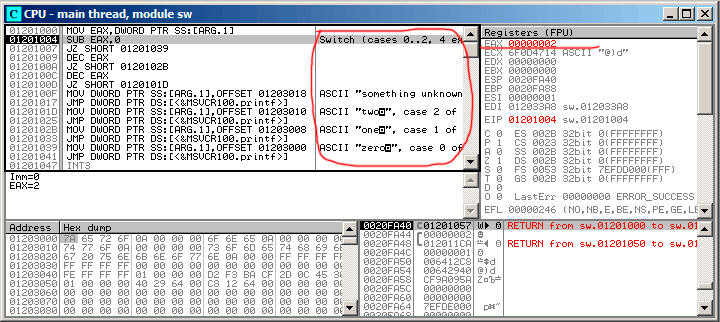
\includegraphics[scale=\FigScale]{patterns/08_switch/1_few/few_olly1.png}
\caption{\olly: \EAX \RU{содержит первый (и единственный) аргумент ф-ции}
\EN{now contain first (and sole) function argument}}
\label{fig:switch_few_olly1}
\end{figure}

\begin{figure}[H]
\centering
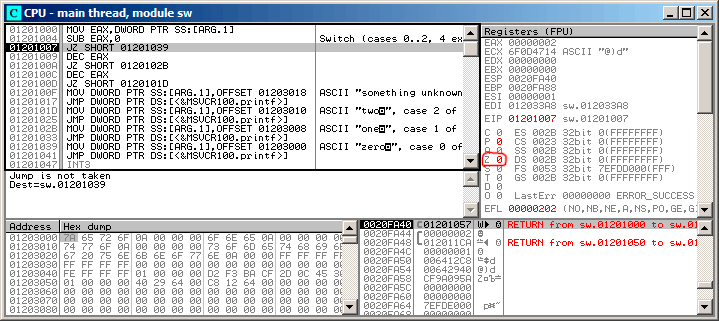
\includegraphics[scale=\FigScale]{patterns/08_switch/1_few/few_olly2.png}
\caption{\olly: \SUB \RU{исполнилась}\EN{executed}}
\label{fig:switch_few_olly2}
\end{figure}

\begin{figure}[H]
\centering
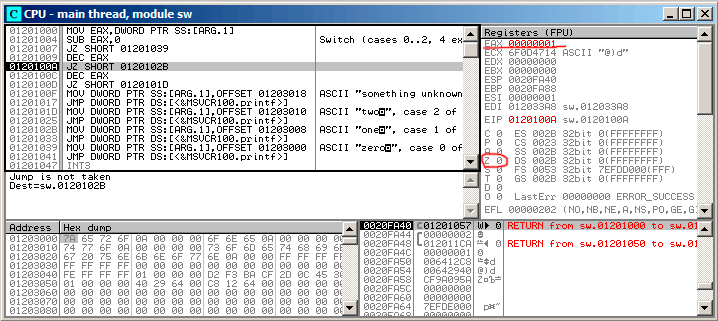
\includegraphics[scale=\FigScale]{patterns/08_switch/1_few/few_olly3.png}
\caption{\olly: \RU{первая}\EN{first} \DEC \RU{исполнилась}\EN{executed}}
\label{fig:switch_few_olly3}
\end{figure}

\begin{figure}[H]
\centering
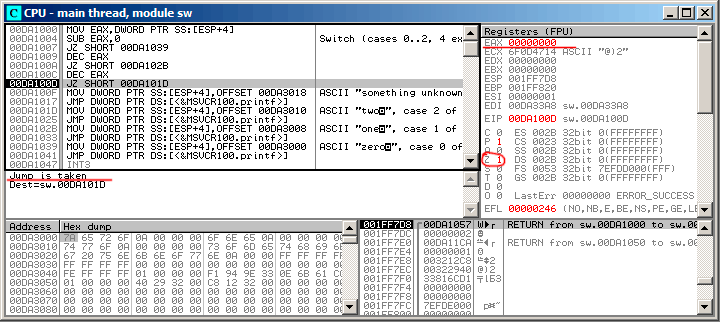
\includegraphics[scale=\FigScale]{patterns/08_switch/1_few/few_olly4.png}
\caption{\olly: \RU{вторая}\EN{second} \DEC \RU{исполнилась}\EN{executed}}
\label{fig:switch_few_olly4}
\end{figure}

\begin{figure}[H]
\centering
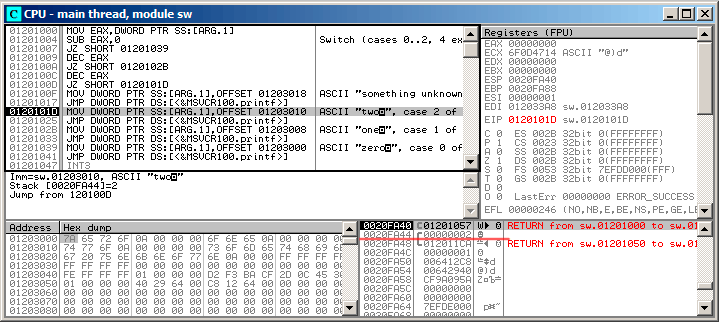
\includegraphics[scale=\FigScale]{patterns/08_switch/1_few/few_olly5.png}
\caption{\olly: \RU{указатель на строку сейчас запишется на место первого аргумента}
\EN{pointer to the string is to be written at the place of first argument}}
\label{fig:switch_few_olly5}
\end{figure}

\begin{figure}[H]
\centering
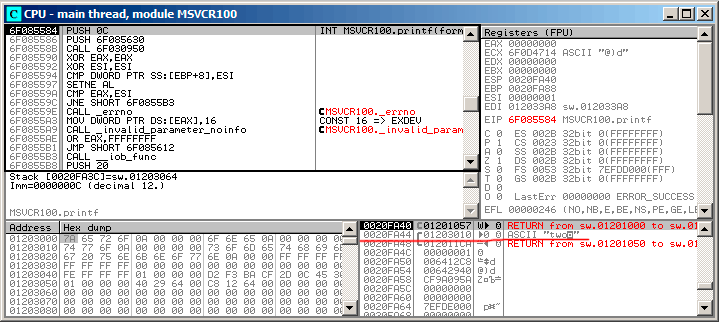
\includegraphics[scale=\FigScale]{patterns/08_switch/1_few/few_olly6.png}
\caption{\olly: \RU{первая инструкция в}\EN{first instruction of} \printf \InENRU MSVCR100.DLL}
\label{fig:switch_few_olly6}
\end{figure}

\begin{figure}[H]
\centering
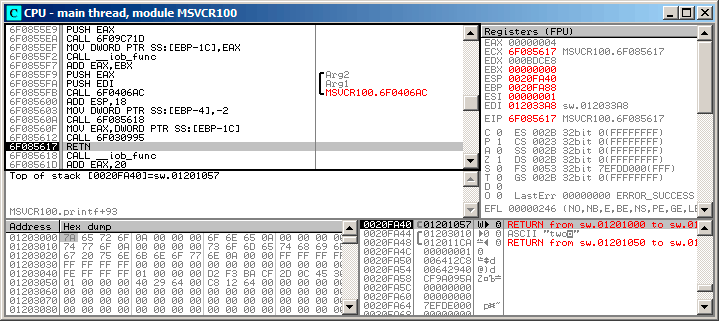
\includegraphics[scale=\FigScale]{patterns/08_switch/1_few/few_olly7.png}
\caption{\olly: \RU{последняя инструкция в}\EN{last instruction of} \printf \InENRU MSVCR100.DLL}
\label{fig:switch_few_olly7}
\end{figure}

\begin{figure}[H]
\centering
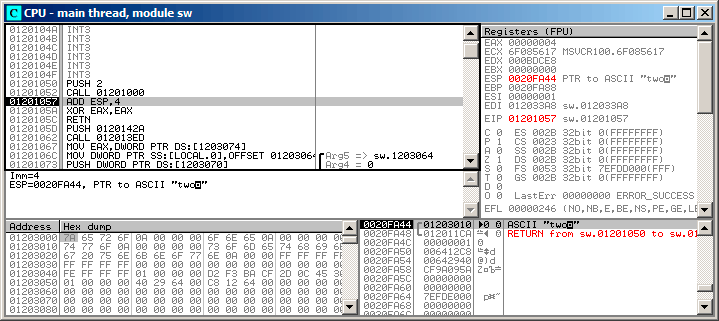
\includegraphics[scale=\FigScale]{patterns/08_switch/1_few/few_olly8.png}
\caption{\olly: \RU{возврат в}\EN{return to} \main}
\label{fig:switch_few_olly8}
\end{figure}

